\section{Relation to the Real Sieve}
For a real 2-gap $(a,a+2)$ and incoming prime $r$, the harmful copies are not chosen freely. They are fixed by
\begin{equation*}
K_{a,r}^{\mathrm{real}}
=
\{-aM^{-1},-(a+2)M^{-1}\}\pmod r.
\end{equation*}
Different parents are coupled through this single arithmetic rule. The real filter has neither independent policy coins nor freely allocated protective and adversarial labels. It nevertheless has directly measurable local destruction $\widehat f_r$, a relative factor $\widehat w_r=r\widehat f_r/2$, and, for a fixed cohort, observed hazard $\widehat D(Q)$. These are the empirical quantities of Section~3.2, not probabilities assigned to the deterministic sieve. Assigning it an effective policy share $\alpha_r$ requires an additional declared companion benchmark, while assessing its positional concentration requires the separate hit count and targeting normalization from Section~6.2.
The relative factor defined in Section~3.2 provides a finite-transition destruction normalization. Section 6.2 adds the allocation question: for the same global destruction budget, how close is the realized local hit count to the uniform mean or targeted maximum?
The companion diagrams identify what a transfer theorem would need to control:
- the observed relative damage $\widehat w_r$ and fixed-cohort hazard $\widehat D(Q)$, together with a separate theorem relating them to candidate conditional hazards; - the exact-quota fractions $u_r$ and their cumulative deviation from $\sum_{r < Q}1/r$; - raw endpoint preference $\beta_r$, quota-normalized effective skew $\kappa_r^{\mathrm{eff}}$, and cumulative skew hazard $D_{\kappa}(Q)$; - any scheduled or effective policy budget $A(Q)$ used for a particular companion specialization; - the availability and abundance premises for the chosen target; and - a deterministic discrepancy bound comparing the real head indicators $I_Q$ with the divergent companion reference weights $\rho_Q$, as formalized in Section~10.
\subsection{Finite Empirical Comparison With Random}
We can compare the real sieve with the random companion at two square-window scales. The first comparison counts the 2-gaps already present in each sequence's own window. For head $h$, let $G_{\mathrm{real}}(h)$ be the number of real 2-gap starts in $[h,h^2)$. The random companion expectation is
\begin{equation*}
E_{\mathrm{random}}(h)
=(h^2-h)\frac12
\prod_{3\le r < h}\left(1-\frac2r\right).
\end{equation*}
The $c=1$ square-window frontier adds the logarithmic excess hazard from Section~3.5:
\begin{equation*}
E_{c=1}(h)
=E_{\mathrm{random}}(h)
\prod_{7\le r < h}
\left(1-\frac{2\log r}{r-2}\right).
\end{equation*}
The figure compares these two expectations with the real count in every fully covered sequence window. Across 188 heads from $3$ through $1129$, the mean ratio $G_{\mathrm{real}}/E_{\mathrm{random}}$ is $0.967$. At the largest covered head it is $0.947$: the real window contains $10{,}056$ 2-gaps, compared with a random expectation of $10{,}616$. The corresponding $c=1$ frontier expectation is only $0.0845$. Over this finite range, the real square-window population follows the random scale and remains far above the square-window failure frontier.
\begin{figure}[htbp]
\centering
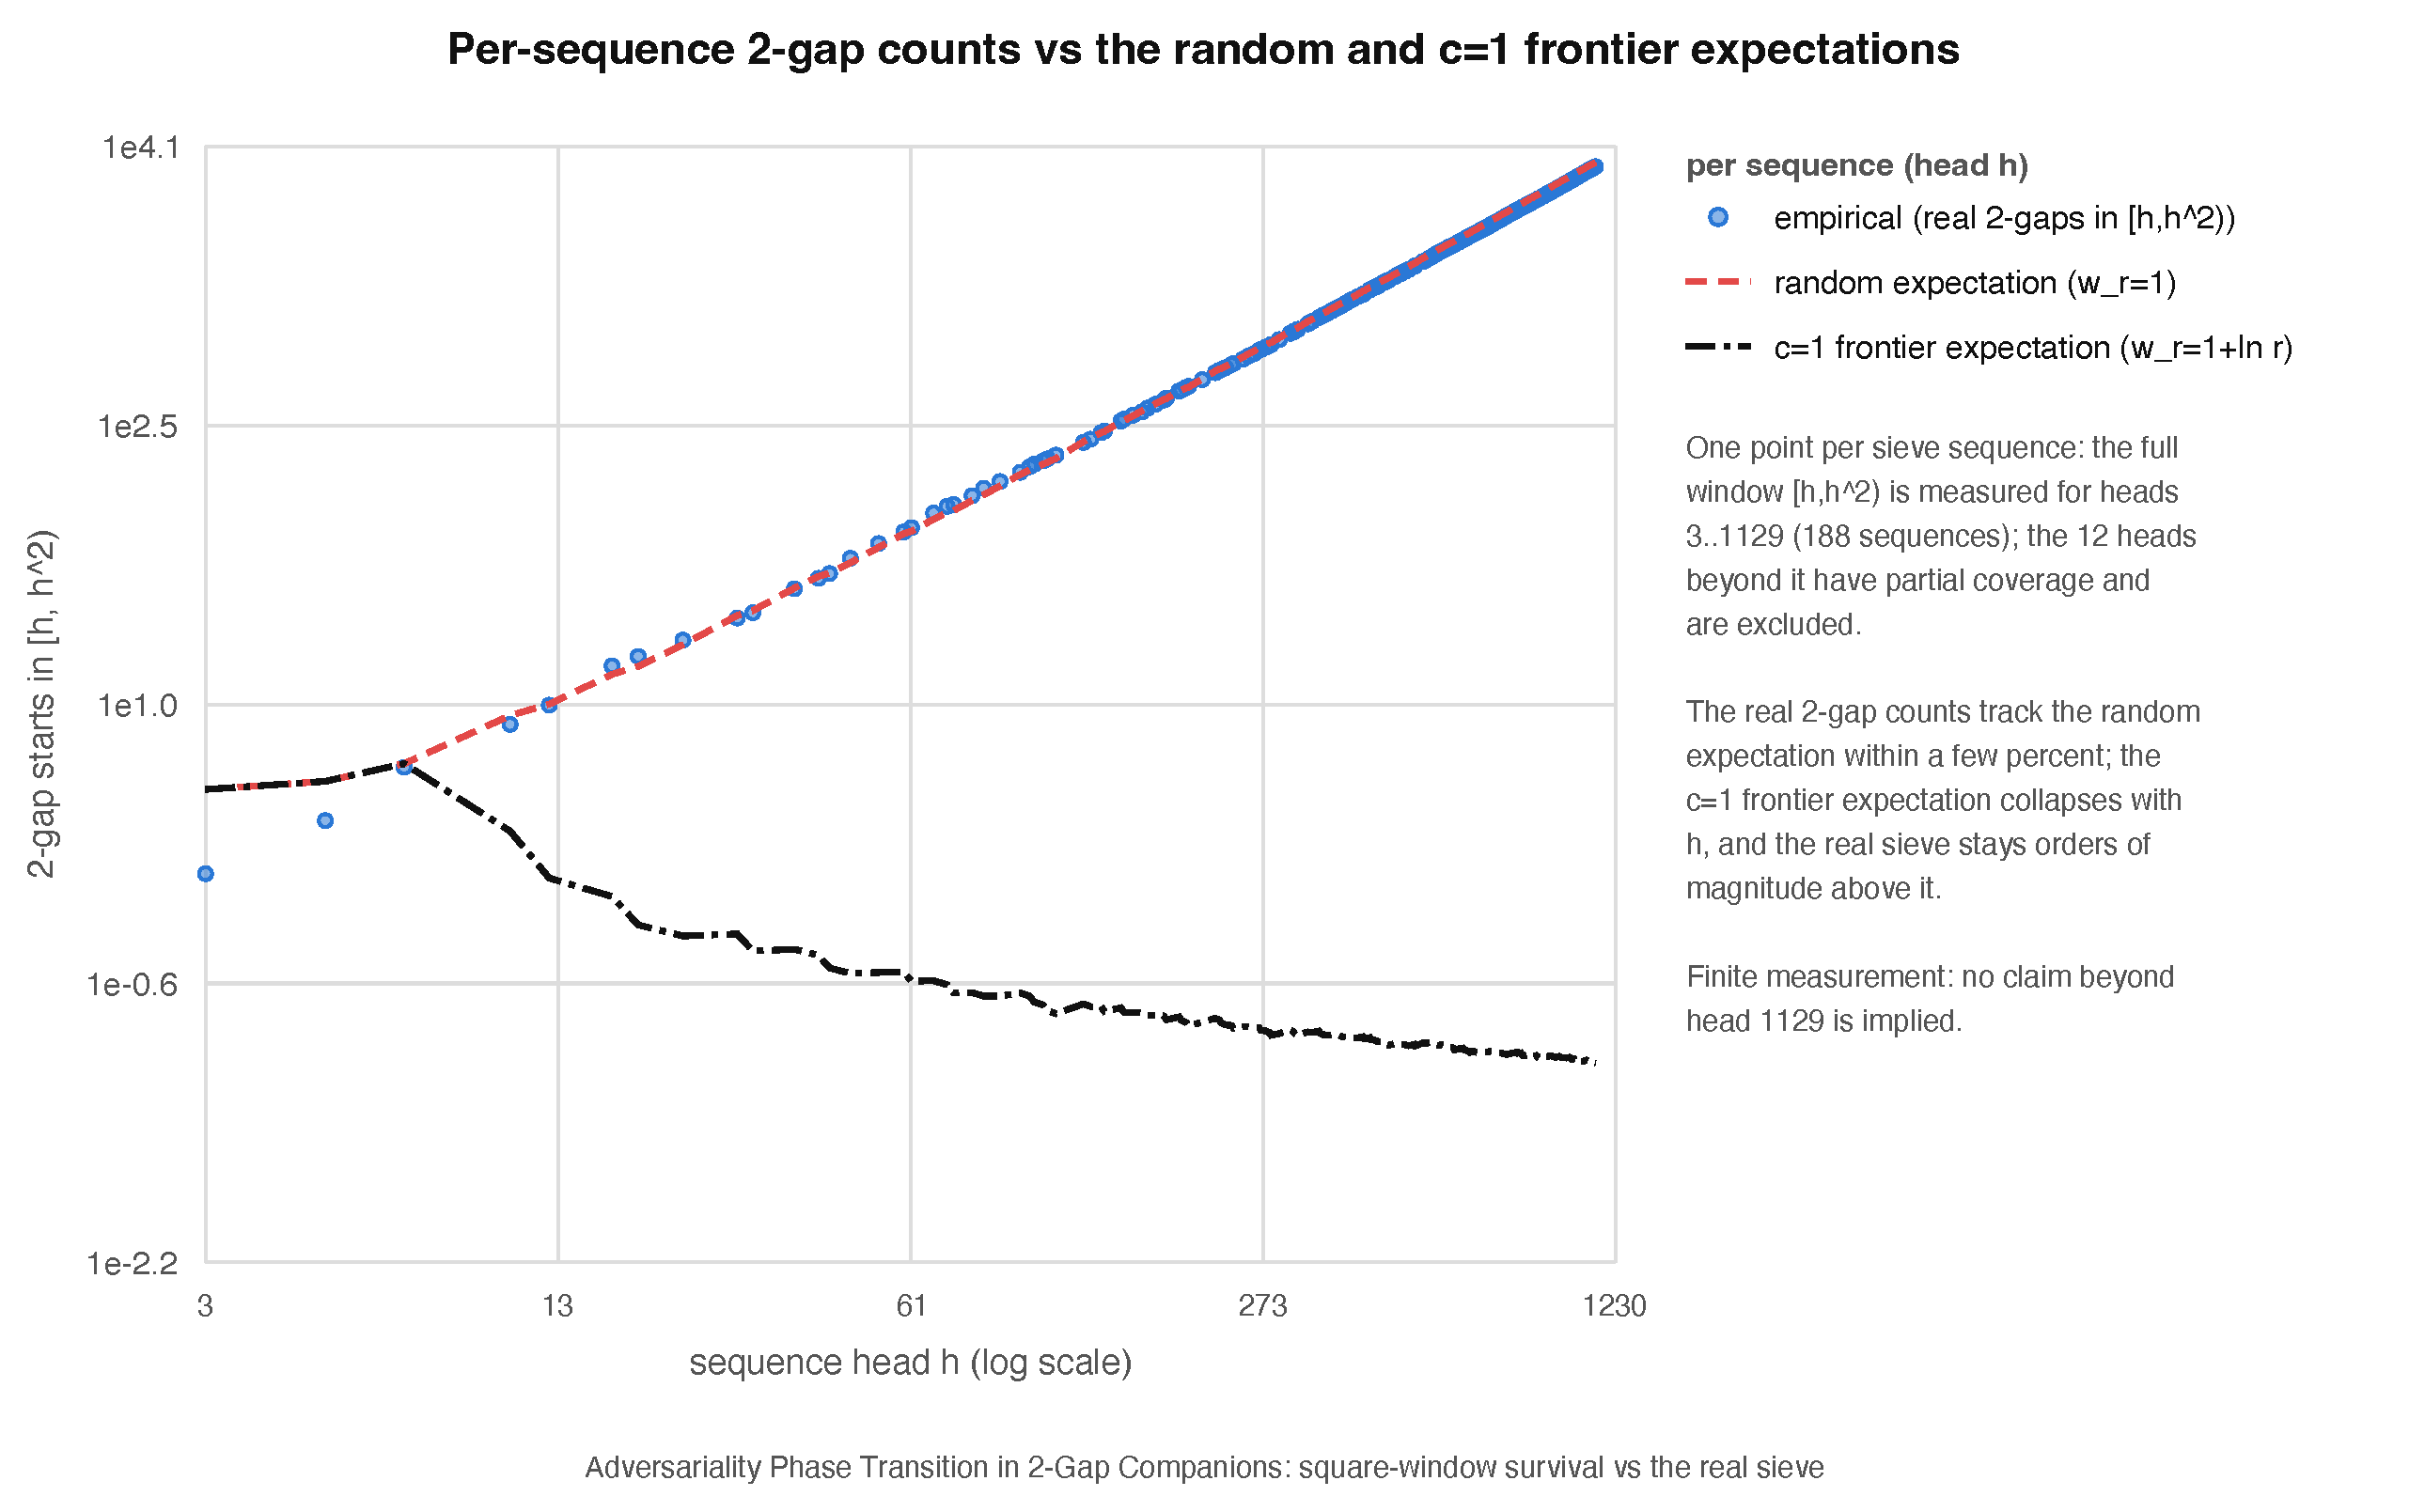
\includegraphics[width=\textwidth]{figures/per-sequence-frontier.pdf}
\caption{Real per-sequence square-window 2-gap counts compared with the random expectation and the c=1 square-window frontier}
\end{figure}
The figure is generated by the \href{https://github.com/thiagomata/prime-numbers/blob/master/python/src/sieve_sequence/per_sequence_frontier_chart.py}{per-sequence frontier calculation} from the \href{https://github.com/thiagomata/prime-numbers/blob/master/data/sieve-sequence/first_gaps_per_seq.csv}{per-sequence survivor data}.
The second comparison isolates one transition. For consecutive primes $p<q$, let $G_p$ be the pre-filter 2-gap population in $[q,q^2)$ and let $H_p$ be the number destroyed when filter $p$ is installed. The observed fraction and its relative factor are
\begin{equation*}
f_p^{\mathrm{real}}:=\frac{H_p}{G_p},
\qquad
w_p^{\mathrm{real}}:=\frac{pf_p^{\mathrm{real}}}{2}.
\end{equation*}
The chart compares $f_p^{\mathrm{real}}$ with the random rate $2/p$ and the $c=1$ square-window boundary $2(1+\log p)/p$. Among 187 distinct measured transitions from $p=3$ through $p=19{,}429$, 186 lie below the random rate and the remaining transition, $p=3$, equals it. Ninety-five transitions destroy no 2-gap in the measured window. From $p\ge1000$, the largest observed relative factor is
\begin{equation*}
w_p^{\mathrm{real}}=0.0523.
\end{equation*}
Thus the measured real transition is not slightly more destructive than the random filter; on these windows it is substantially less destructive.
\begin{figure}[htbp]
\centering
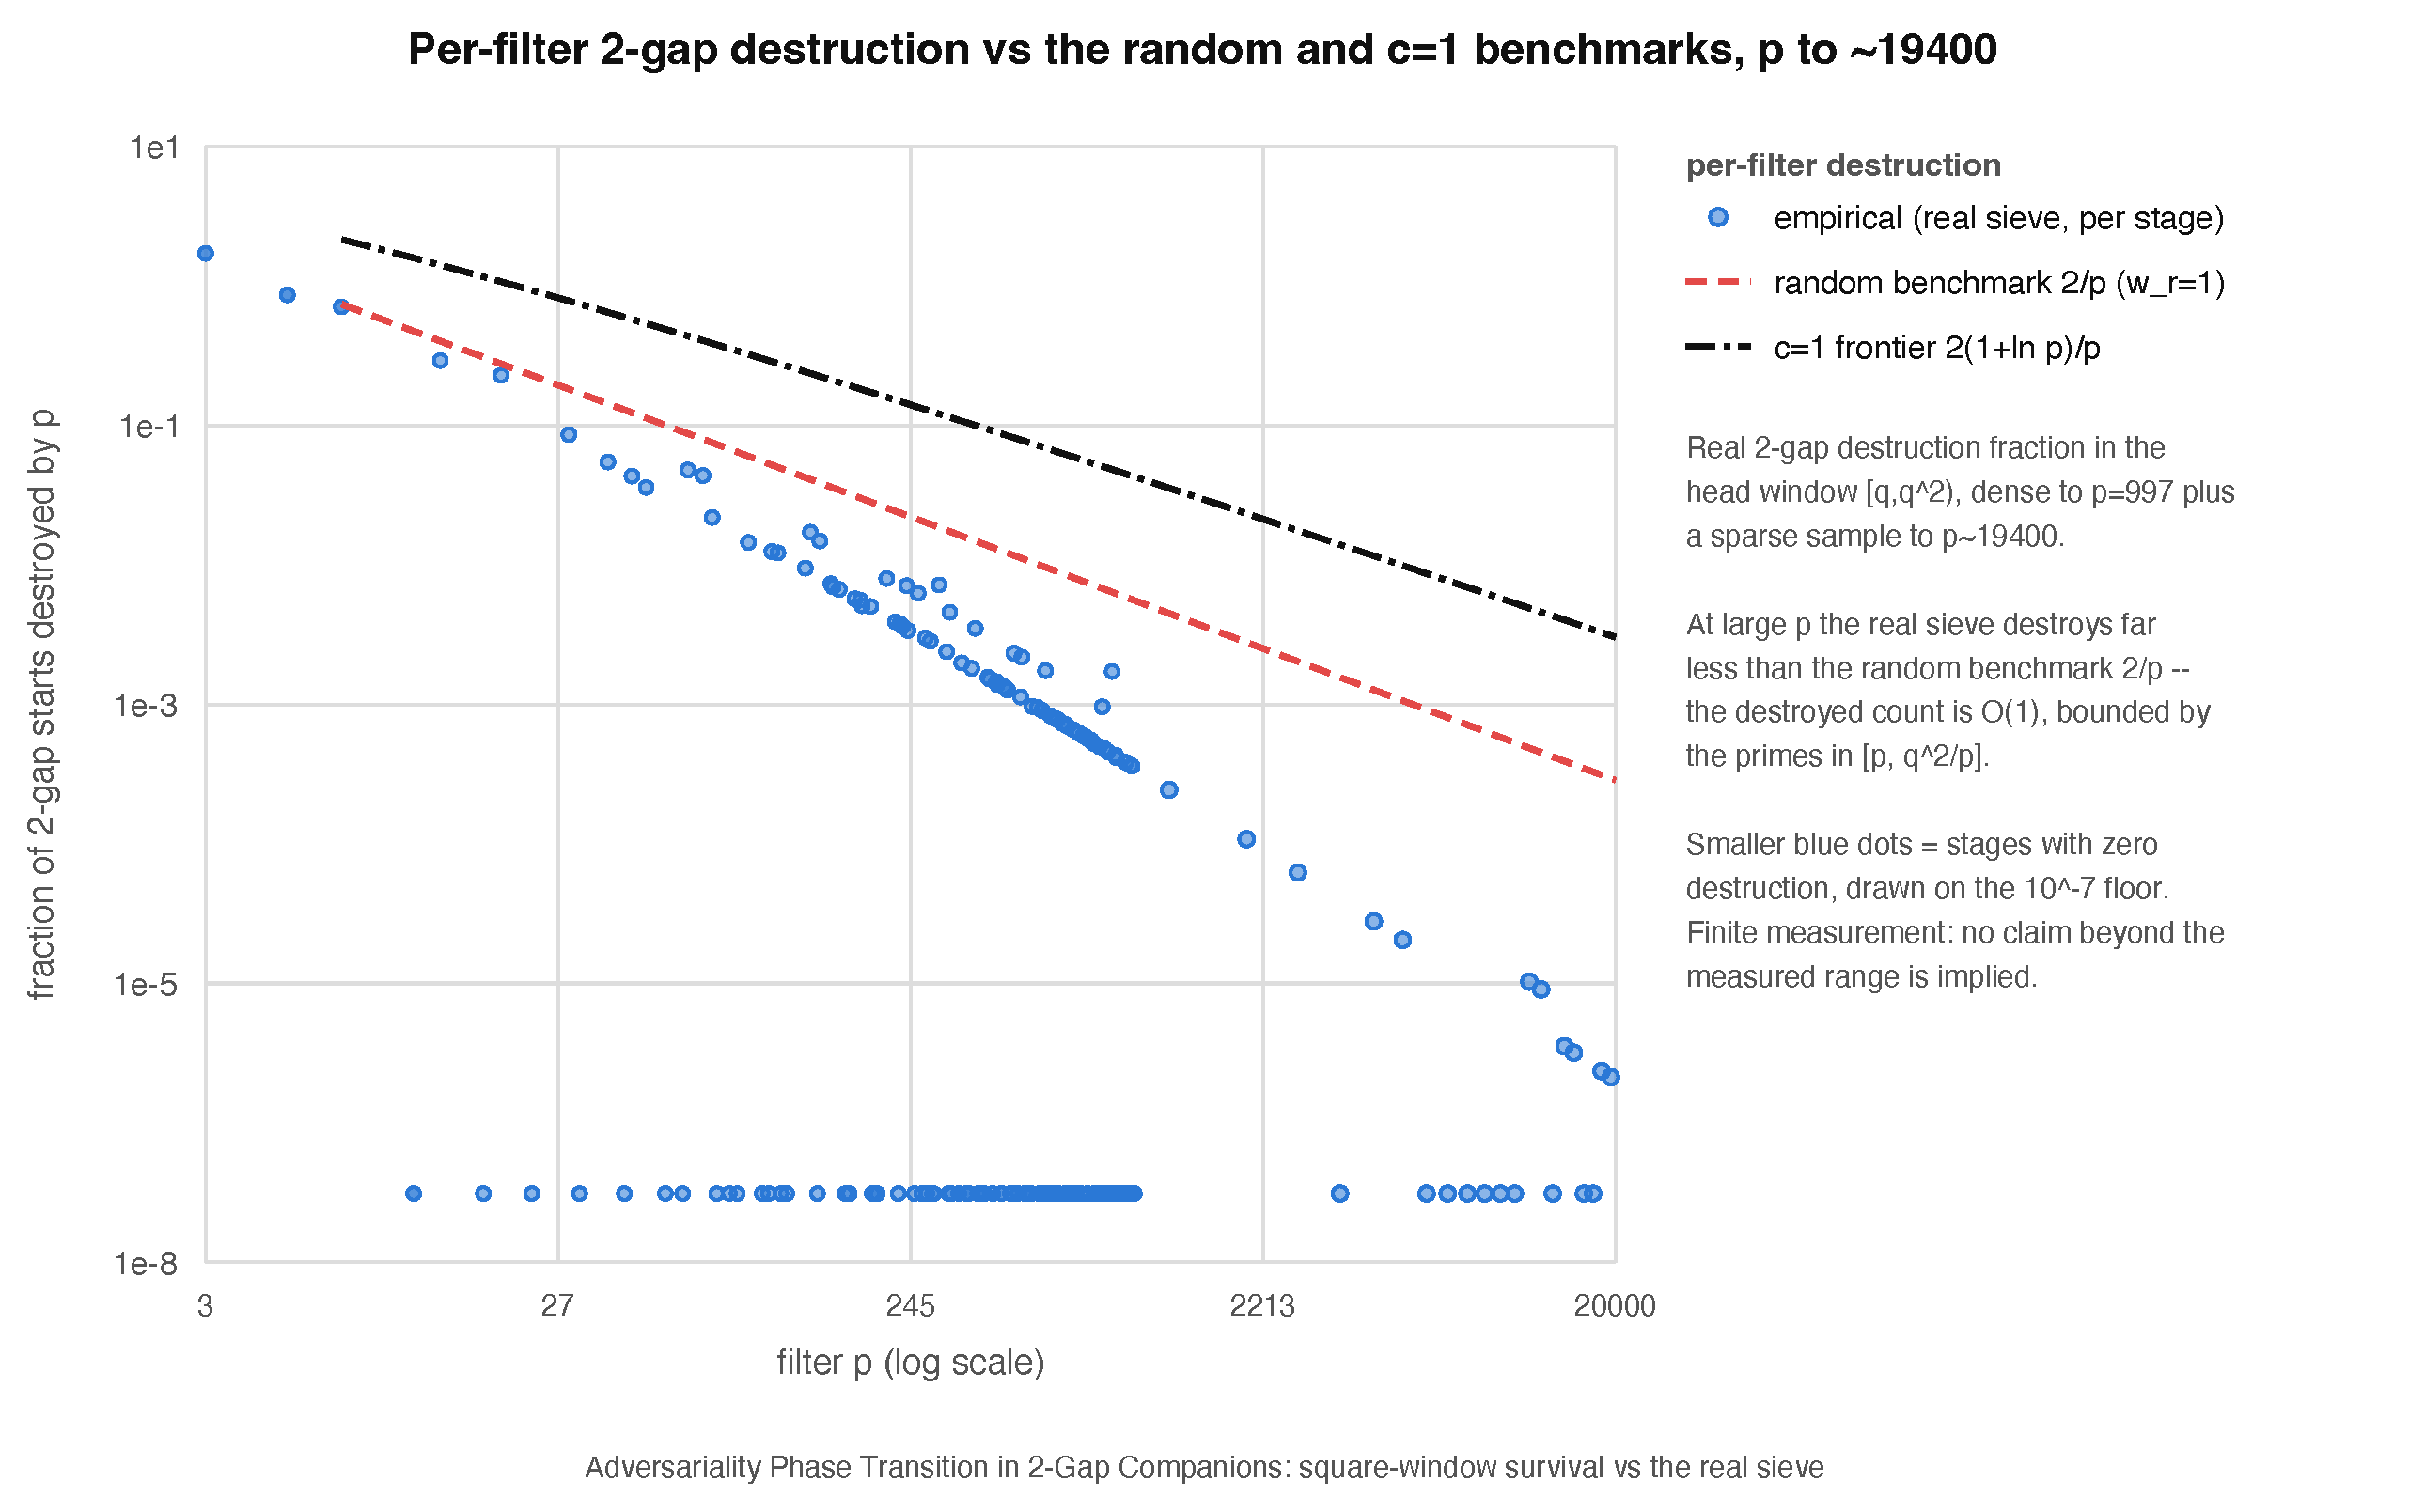
\includegraphics[width=\textwidth]{figures/frontier-comparison-stages.pdf}
\caption{Real per-transition square-window 2-gap destruction compared with the random rate and the c=1 square-window boundary}
\end{figure}
The figure is generated by the \href{https://github.com/thiagomata/prime-numbers/blob/master/python/src/sieve_sequence/frontier_comparison_stages_chart.py}{per-transition frontier calculation} from the \href{https://github.com/thiagomata/prime-numbers/blob/master/data/candidates/window-measurements.csv}{dense} and \href{https://github.com/thiagomata/prime-numbers/blob/master/data/candidates/window-measurements-sparse.csv}{sparse} transition data. Zero-destruction transitions are displayed on the chart's $10^{-7}$ floor so that they remain visible on a logarithmic axis.
The two findings are compatible. The first chart measures the population left after all earlier filters; the second isolates the next filter acting on a new window. Neither dataset follows one fixed cohort through every filter below a single head, so their changing-window fractions cannot be multiplied into one cumulative hazard.
The complete modular cycle supplies an exact reference in two complementary views. The first is local to one filter: it asks what fraction of the expanded cyclic population that filter destroys. The second is cumulative: it asks how much of a normalized starting population remains after those one-filter fractions are compounded. The two figures below deliberately mirror these two steps of the calculation.
\subsubsection*{Exact Per-Filter Destruction}
If $T$ old cyclic 2-gaps are expanded through a new prime $r$, there are $rT$ copies and exactly two harmful copy indices per parent. Consequently,
\begin{equation*}
\begin{aligned}
H_r^{\mathrm{cycle}}
&=2T
&&[\text{Two Harmful Copy Classes}],\\
f_r^{\mathrm{cycle}}
&=\frac{H_r^{\mathrm{cycle}}}{rT}
=\frac2r
&&[\text{Substitution}],\\
w_r^{\mathrm{cycle}}
&=1,
&&[\text{By Definition}],\\
D_{\mathrm{cycle}}(R)-D_{\mathrm{random}}(R)
&=0.
&&[\text{Termwise Equality; Q.E.D.}]
\end{aligned}
\end{equation*}
Thus the full-cycle destruction fraction equals the neutral benchmark as a count identity. This does not say that the harmful positions are independently random. The figure below makes the identity visible alongside the $c=1$ reference on the valid range $29\le r\le251$. Its simplicity is the point: the overlap between the exact-cycle and neutral curves is the graphical form of the algebra above, while the separated $c=1$ curve shows the scale of the hypothetical logarithmic worsening. The chart is strong precisely because the reader can verify the stated relationship without additional interpretation.
\begin{figure}[htbp]
\centering
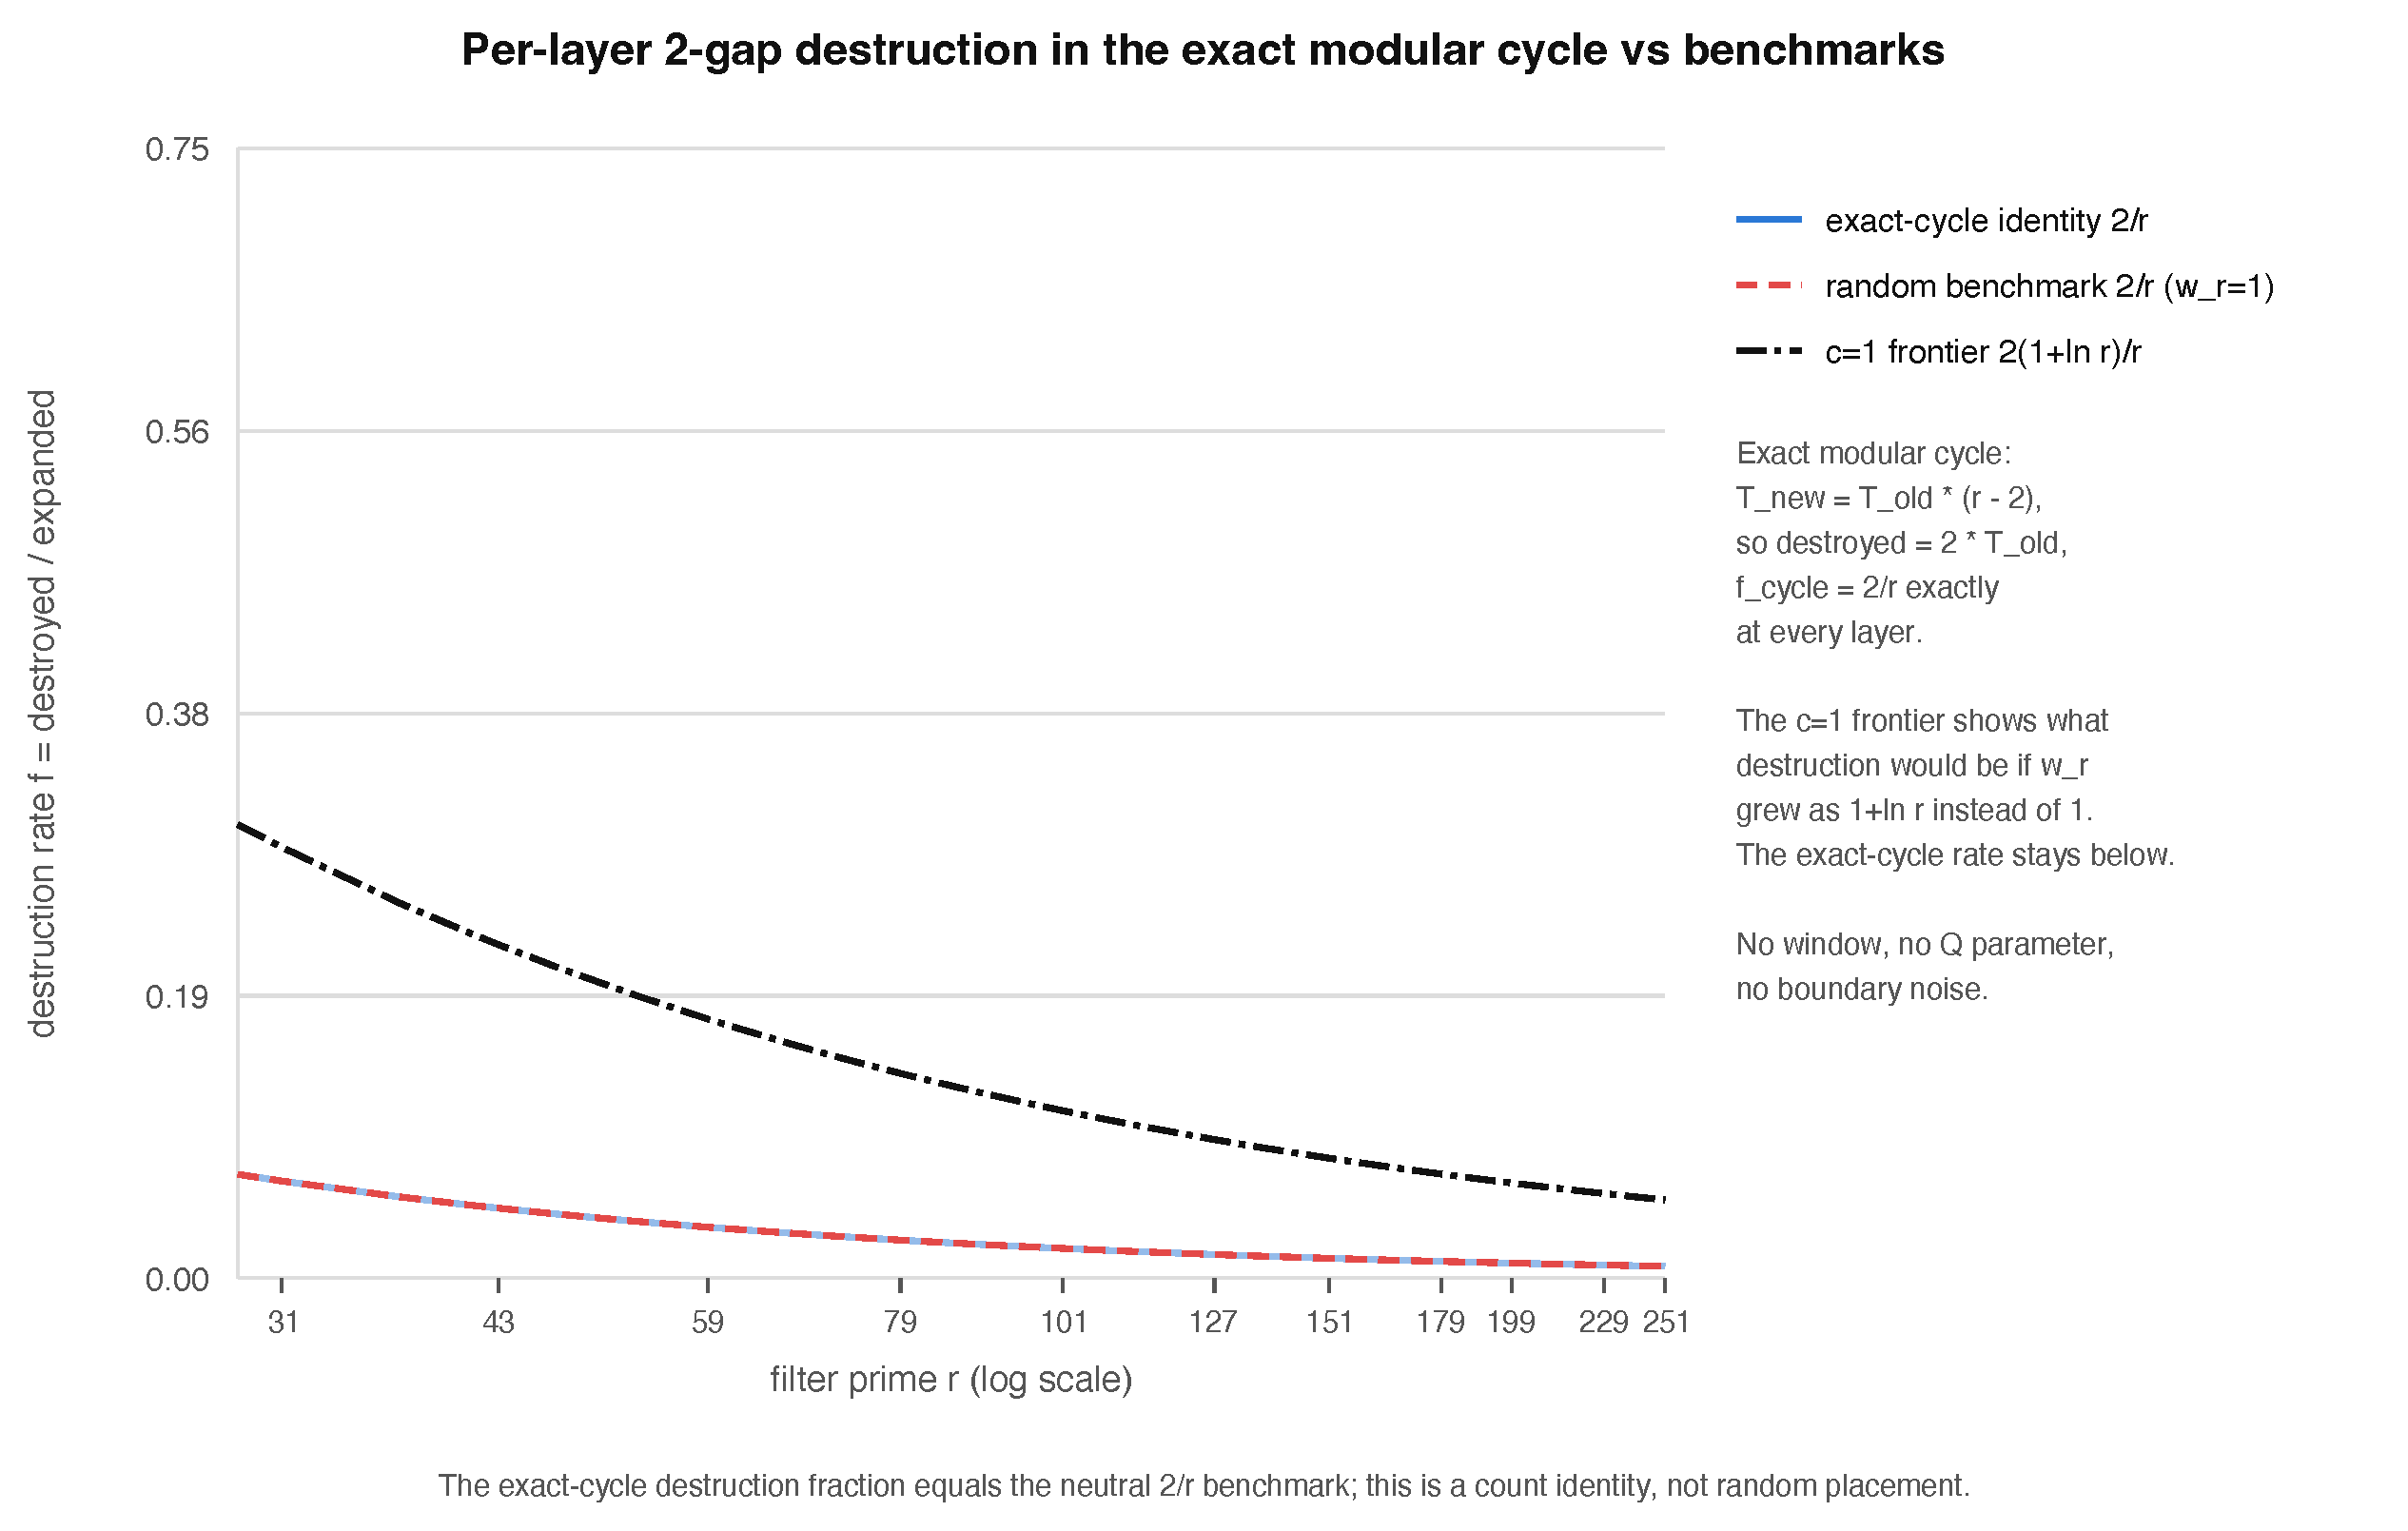
\includegraphics[width=\textwidth]{figures/full-cycle-destruction.pdf}
\caption{Exact full-cycle 2-gap destruction fraction compared with the neutral rate and the c=1 reference}
\end{figure}
The figure is generated by the \href{https://github.com/thiagomata/prime-numbers/blob/master/python/src/sieve_sequence/full_cycle_destruction_chart.py}{full-cycle destruction calculation}. The underlying two-class result is proved in \href{https://github.com/thiagomata/prime-numbers/blob/master/articles/chapter6/gap-dynamics.md#61-one-new-prime-forbids-two-copy-classes}{Gap Dynamics \S{}6.1} \cite{gapdynamics2026}.
\subsubsection*{Cumulative Survival Consequence}
The first diagram makes the proved one-filter equality visible. Compounding those same factors gives the normalized complete-cycle survival reference
\begin{equation*}
\begin{aligned}
P_{\mathrm{cycle}}(29,R)
&=\prod_{29\le p\le R}\left(1-\frac2p\right),\\
P_{c=1}(29,R)
&=\prod_{29\le p\le R}
\left(1-\frac{2(1+\log p)}p\right).
\end{aligned}
\end{equation*}
At $R=251$, these normalized products are $0.3733$ and $0.003676$, respectively, a ratio of about $102$. The second figure therefore shows the cumulative consequence that the first figure cannot show by itself: the repeated per-filter separation from the $c=1$ schedule compounds into a separation of more than two orders of magnitude over the plotted range. The anchor $29$ is the first plotted prime and keeps every $c=1$ factor in $(0,1)$; changing a finite anchor changes the normalizing constants, not the asymptotic exponents. This is a reference comparison, not evidence of head recurrence.
\begin{figure}[htbp]
\centering
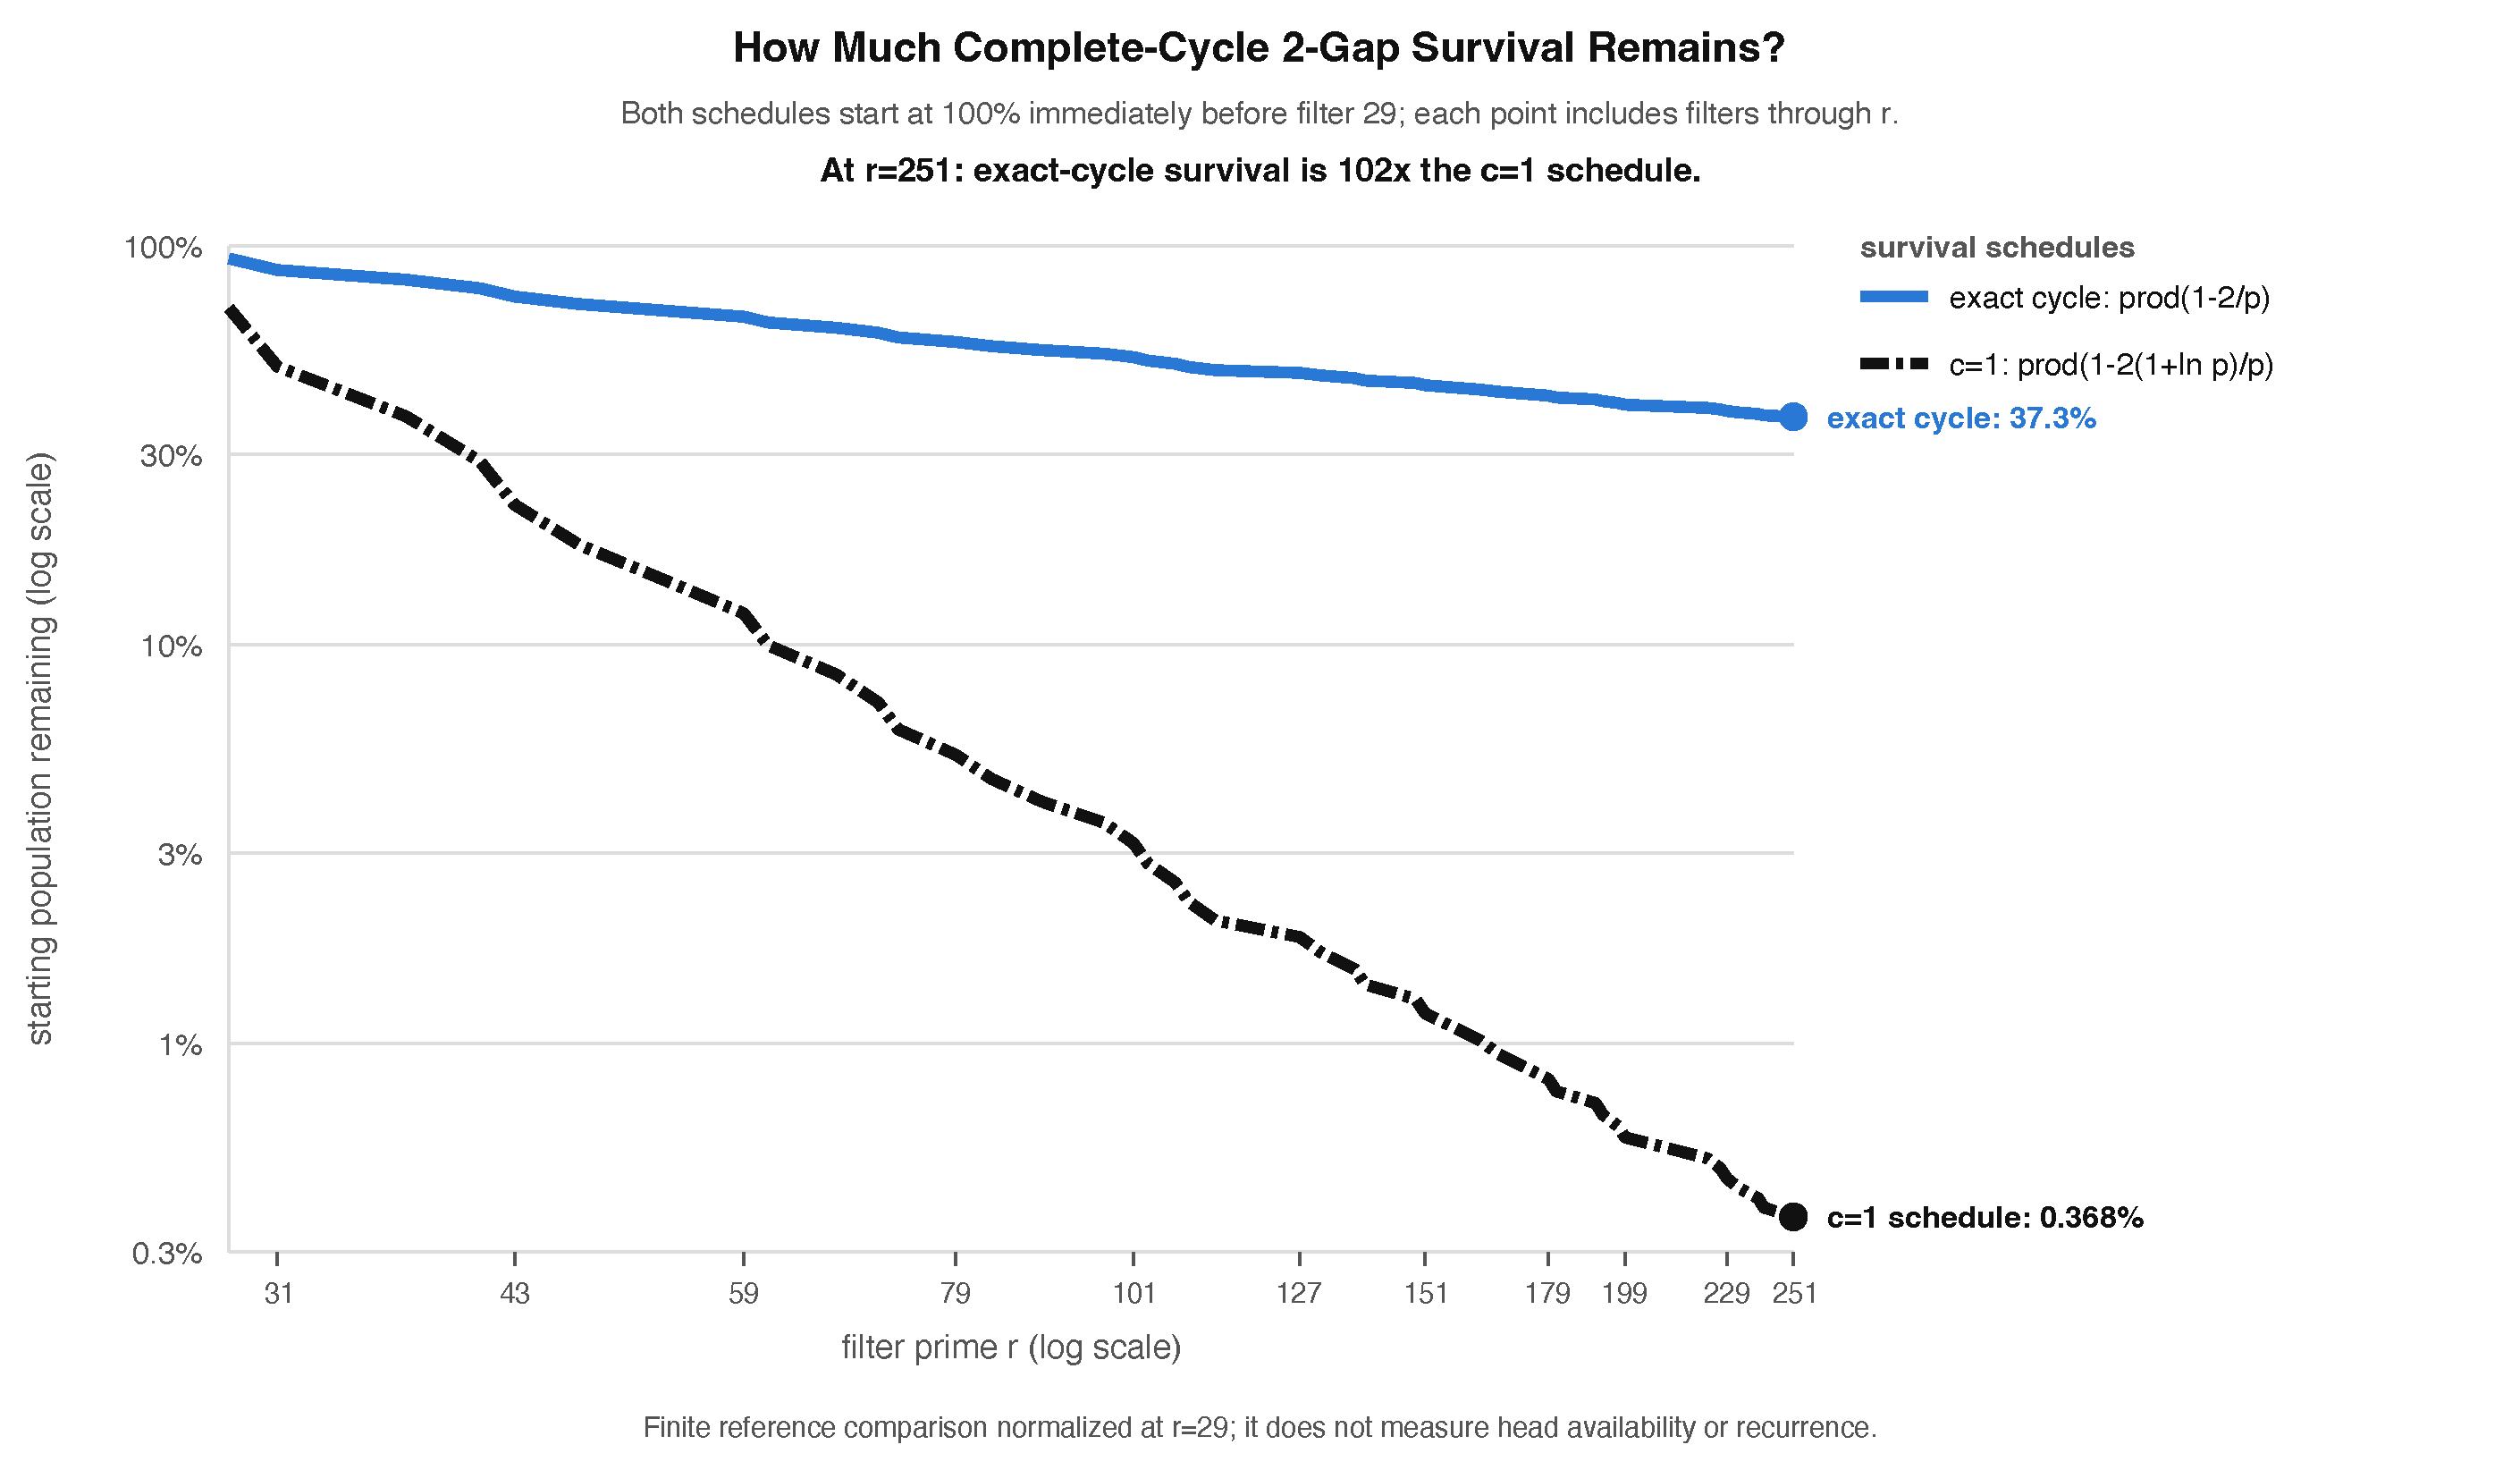
\includegraphics[width=\textwidth]{figures/full-cycle-survival.pdf}
\caption{Normalized full-cycle 2-gap survival under the exact per-filter law compared with the c=1 schedule}
\end{figure}
The figure is generated by the \href{https://github.com/thiagomata/prime-numbers/blob/master/python/src/sieve_sequence/full_cycle_survival_chart.py}{full-cycle survival calculation}.
Read together, the two full-cycle figures give a direct progression from the one-filter identity to its cumulative effect. A separate fixed-cohort experiment then asks the next question: what remains true when a finite window cuts through partial cycles? It follows every 2-gap start initially present in $[Q,Q^2)$ through all filters $r<Q$. Exact set comparisons at $Q=17$ and $Q=101$ confirm that this explicit cohort agrees layer by layer with the maintained Reading A lineage. For
\begin{equation*}
c_{\mathrm{eff}}(r)
:=\frac{\widehat D_{\mathrm{real}}(r)-D_{\mathrm{random}}(r)}{2\log r},
\end{equation*}
the four runs $Q\in\{17,101,251,503\}$ give signed values between $-0.0353$ and $0.00908$. The largest positive value is $0.00907$ at $Q=251$; among the two larger runs, all absolute values are at most $0.00908$. Because the complete-cycle excess is exactly zero, the deviations arise when the fixed interval cuts partial cycles. Their size and placement remain finite empirical facts; partial-cycle localization can contain the arithmetic difficulty that the complete-cycle identity does not see.
\begin{figure}[htbp]
\centering
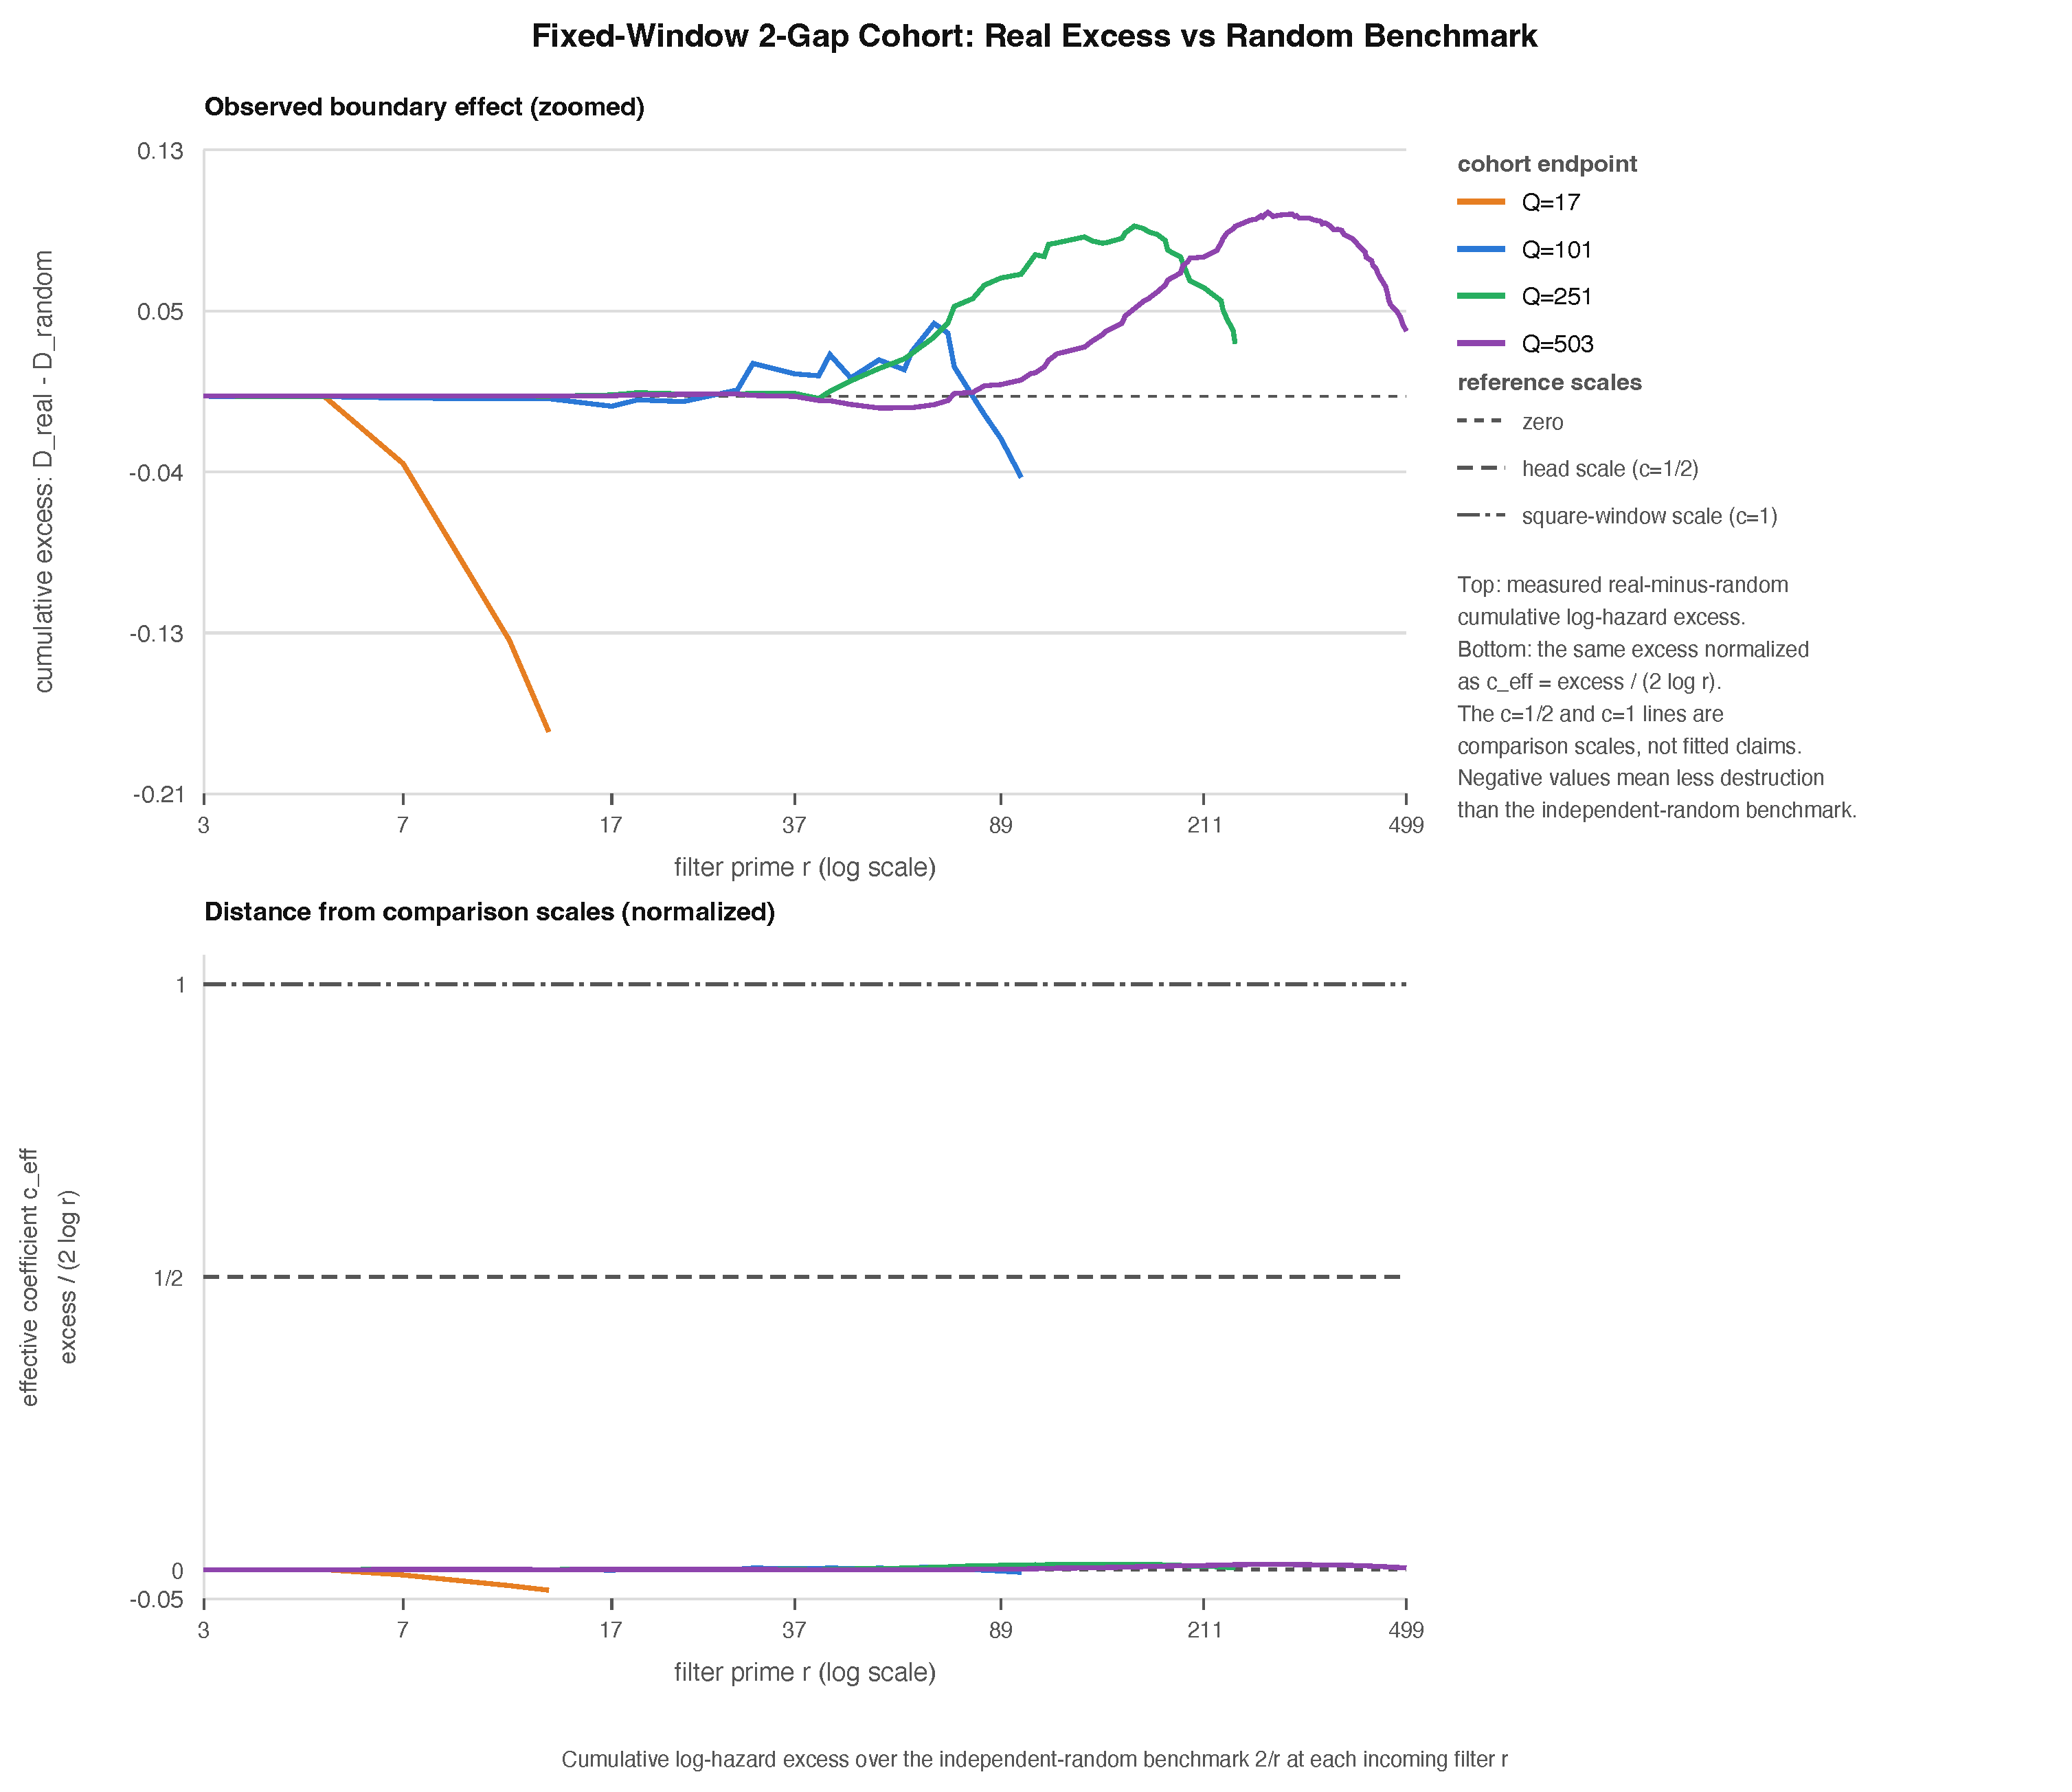
\includegraphics[width=\textwidth]{figures/fixed-lineage-hazard.pdf}
\caption{Cumulative hazard of fixed-window 2-gap cohorts for four finite Q values}
\end{figure}
The figure is generated by the \href{https://github.com/thiagomata/prime-numbers/blob/master/python/src/sieve_sequence/fixed_lineage_hazard_chart.py}{fixed-lineage hazard calculation} from the dedicated fixed-cohort CSVs. Its value is a robustness check: even in non-aligned finite windows the boundary deviations are small relative to the $c=1/2$ and $c=1$ comparison scales.
None of these measurements follows the distinguished pair at the head. Transferring the head phase diagram still requires an arithmetic theorem that controls coherent CRT-coupled placement together with persistent availability and cross-layer dependence.
